\newpage
\section{Questão 02}
Na segunda questão, um sinal  $x[n]$ é dado conforme a expressão abaixo:
\[
x[n] = 
\begin{cases} 
e^{-\frac{(0.1n)^2}{2}} & \text{se } |n| \leq 50 \\ 
0 & \text{caso contrário}
\end{cases}
\]

Nas etapas seguintes, pretende-se analisar o efeito da subamostragem de um sinal observando a representação em magnitude e em fase dos sinais. 

Subamostragem a cada duas, quatro e cinco amostras foram realizadas.

A Figura \ref{fig:graph_09} contém a representação do sinal em magnitude na qual a amostragem foi feita de forma regular, ou seja, a cada valor de \textit{n}. 

\begin{figure}[!htb]
    \centering
    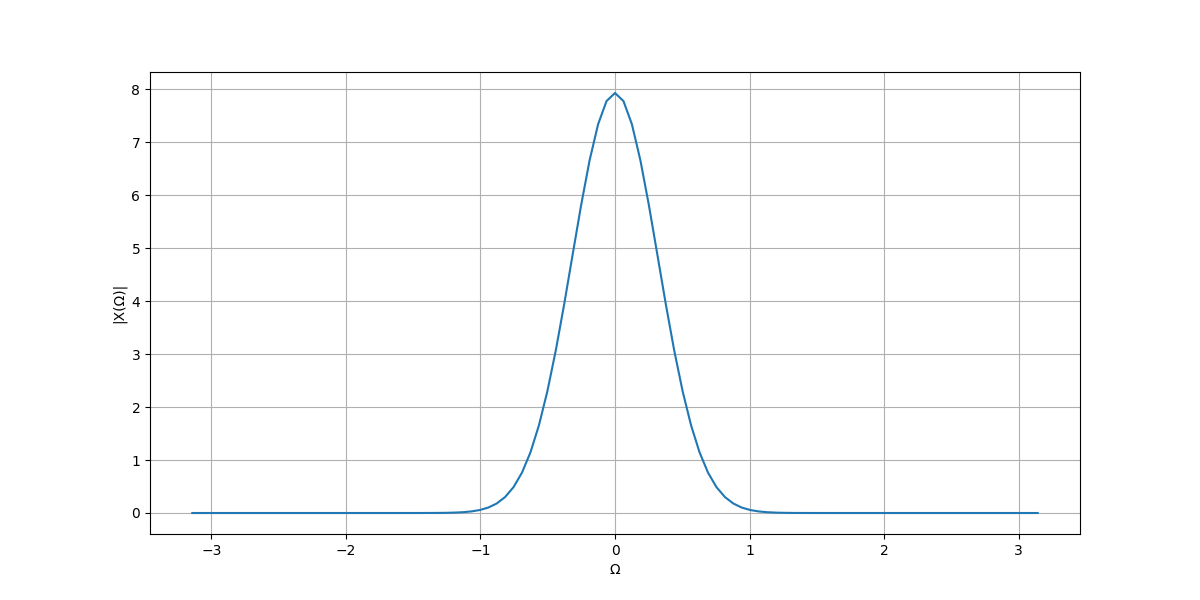
\includegraphics[width=\linewidth]{Imagens/fig09.png}
    \caption{Magnitude para sinal amostrado}
    \label{fig:graph_09}
\end{figure}

Na Figura \ref{fig:graph_09}, pode-se observar algumas características importantes desse sinal que serão modificados conforme a subamostragem é realizada, cada vez a uma taxa maior. 

Portanto, deve-se atentar à amplitude alcançada por esse espectro e a banda alcançada pelo sinal.

\begin{figure}[!htb]
    \centering
    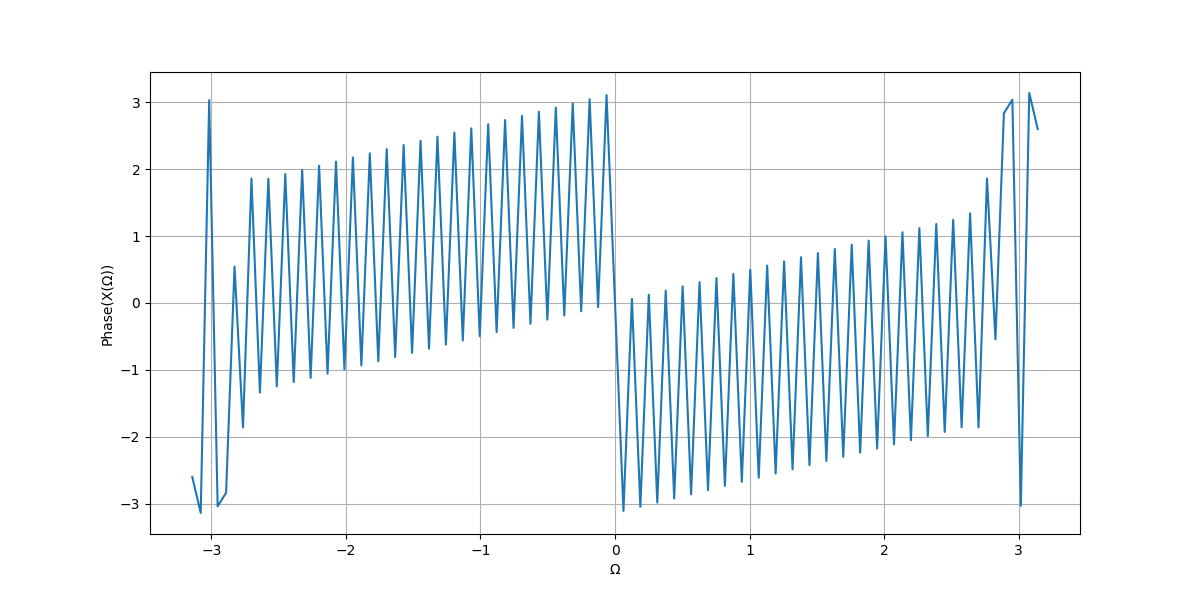
\includegraphics[width=\linewidth]{Imagens/fig10.png}
    \caption{Fase para sinal amostrado}
    \label{fig:graph_10}
\end{figure}

Em relação à fase do sinal, deve-se ficar atento ao efeito que o \textit{aliasing} provoca, focando nas descontinuidades abruptas existentes nessa representação.

Na Figura \ref{fig:graph_11}, percebe-se duas mudanças na magnitude do sinal quanto uma subamostragem de nível dois acontece, ou seja, quando uma amostra é descartada e a seguinte é utilizada, e assim por seguinte.

Percebe-se que a amplitude máxima do espectro decaiu pela metade. Em contrapartida, percebe-se que a banda do sinal aumentou. Uma subamostragem diminui a taxa de amostragem utilizada, de forma prática ao analisar o sinal. Assim, uma compressão do espectro em relação à amplitude é vista. Além disso, distorções serão introduzidas em regiões do espectro nas quais um espectro invade o espectro adjacente. A partir disso, distorções do sinal são introduzidas.

\begin{figure}[!htb]
    \centering
    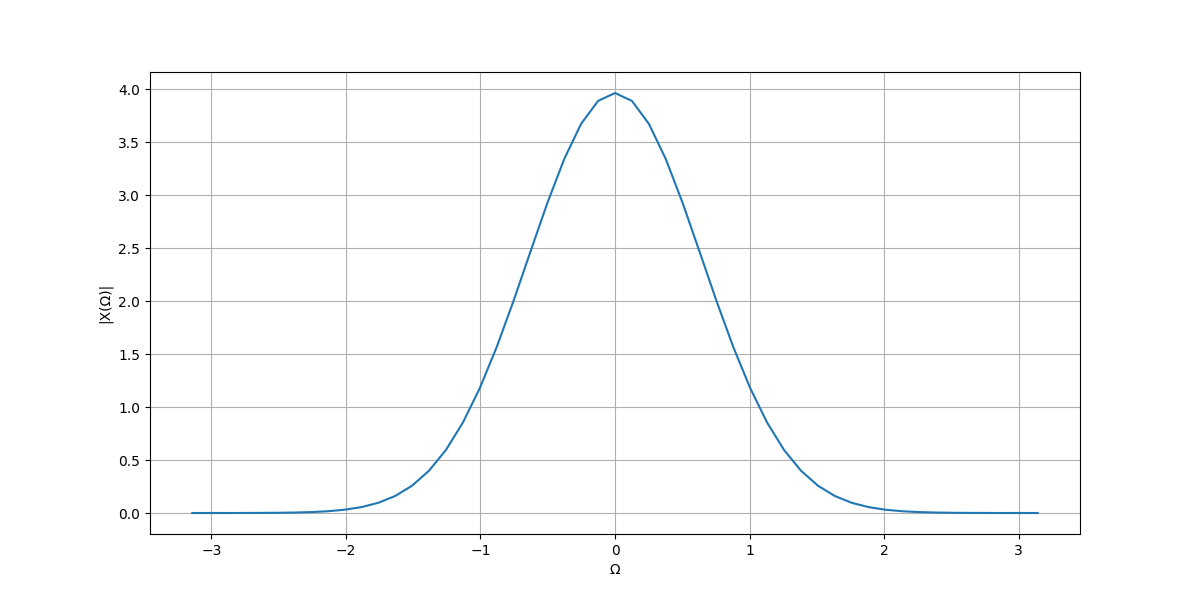
\includegraphics[width=\linewidth]{Imagens/fig11.png}
    \caption{Magnitude para sinal subamostrado a [2n]}
    \label{fig:graph_11}
\end{figure}

Outros efeitos da subamostragem de nível dois são visualizadas em relação à fase do sinal. Dessa forma, como se pode ver na Figura \ref{fig:graph_12}, a fase é afetada pela subamostragem visto que descontinuidades e distorções em frequências replicadas são vistas com mais intensidade. 

\begin{figure}[!htb]
    \centering
    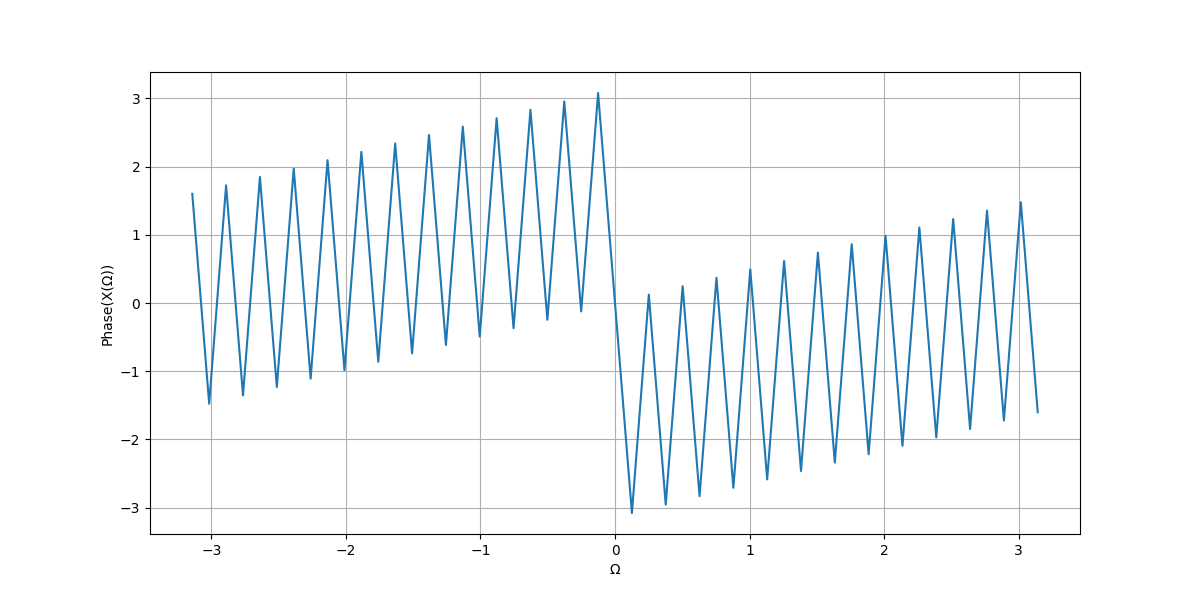
\includegraphics[width=\linewidth]{Imagens/fig12.png}
    \caption{Fase para sinal subamostrado a [2n]}
    \label{fig:graph_12}
\end{figure}

Ao se aumentar o nível da subamostragem, os efeitos citados acima devem se intensificar. 

Conforme se encontra presente na Figura \ref{fig:graph_13}, ao dobrar o nível de subamostragem, de dois para quatro, o mesmo efeito de compressão do espectro em relação a amplitude ocorreu. A amplitude máxima caiu pela metade, enquanto o alcance da banda do espectro se expande. Isso ocorre devido à queda da taxa de amostragem efetiva utilizada nesse sinal, de forma que bandas adjacentes passam a interferir entre si, provocando o efeito que se chama \textit{aliasing}.

\begin{figure}[!htb]
    \centering
    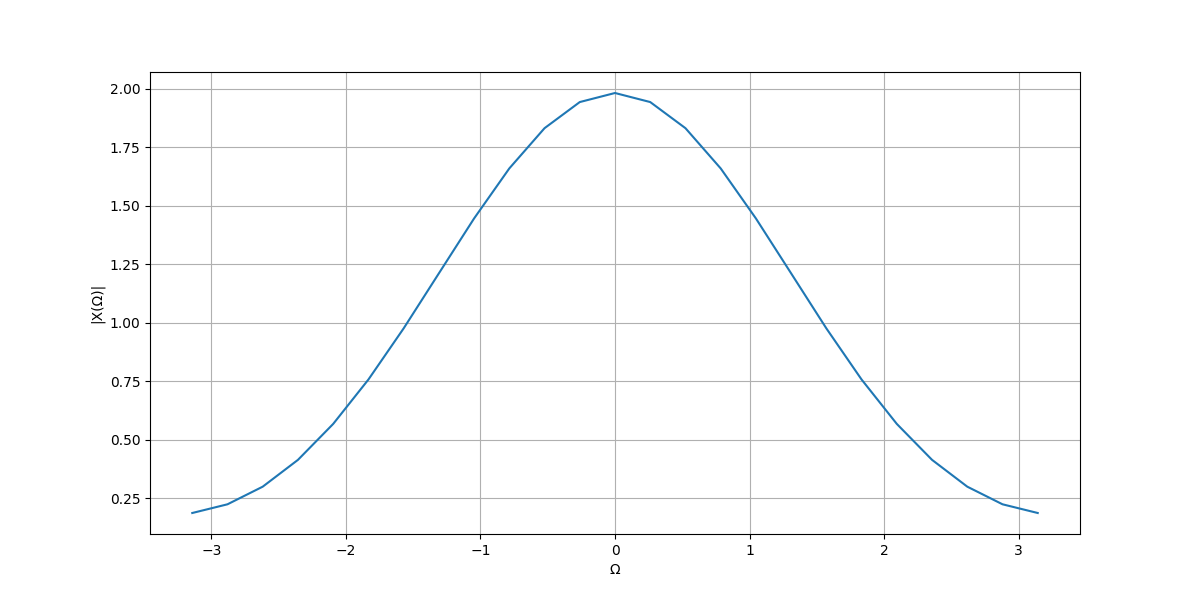
\includegraphics[width=\linewidth]{Imagens/fig13.png}
    \caption{Magnitude para sinal subamostrado a [4n]}
    \label{fig:graph_13}
\end{figure}

Além disso, o mesmo efeito visto na fase da subamostragem nível dois pode ser visualizado na Figura \ref{fig:graph_14} (subamostragem de nível quatro). Assim, observa-se que as descontinuidades da fase se intensificaram, distorcendo ainda mais os sinais.

\begin{figure}[!htb]
    \centering
    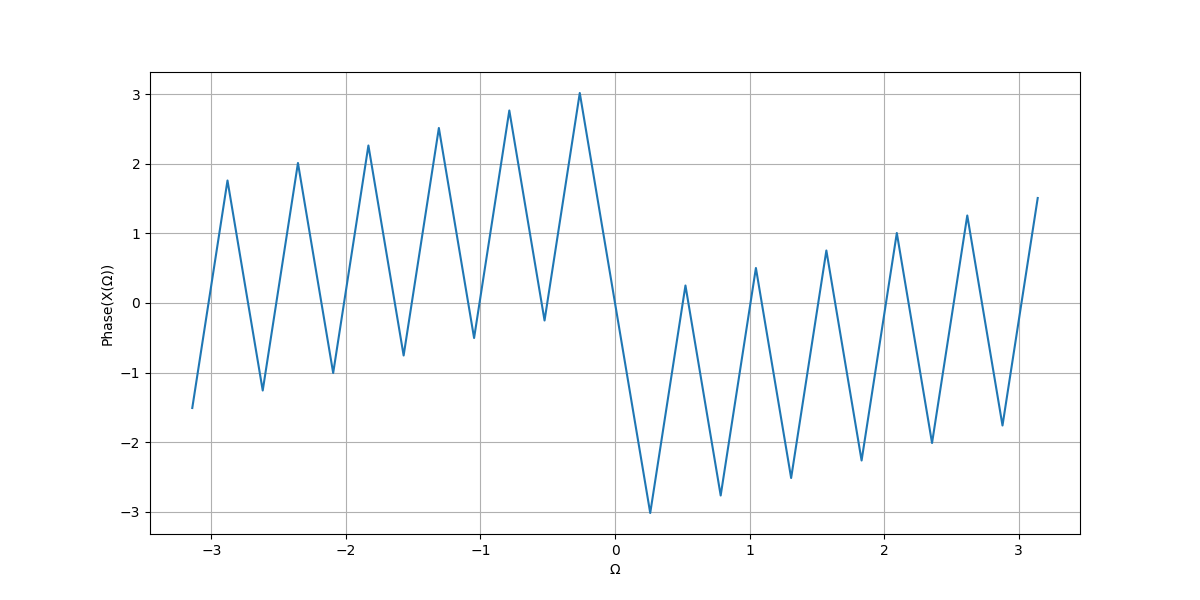
\includegraphics[width=\linewidth]{Imagens/fig14.png}
    \caption{Fase para sinal subamostrado a [4n]}
    \label{fig:graph_14}
\end{figure}

Ao final, tem-se uma subamostragem de nível cinco. Novamente, os efeitos elencados acima são vistos. Na Figura \ref{fig:graph_15}, pode-se observar a compressão do espectro em relação a amplitude e uma expansão do espectro ocasionada pelo fenômeno \textit{aliasing}.

\begin{figure}[!htb]
    \centering
    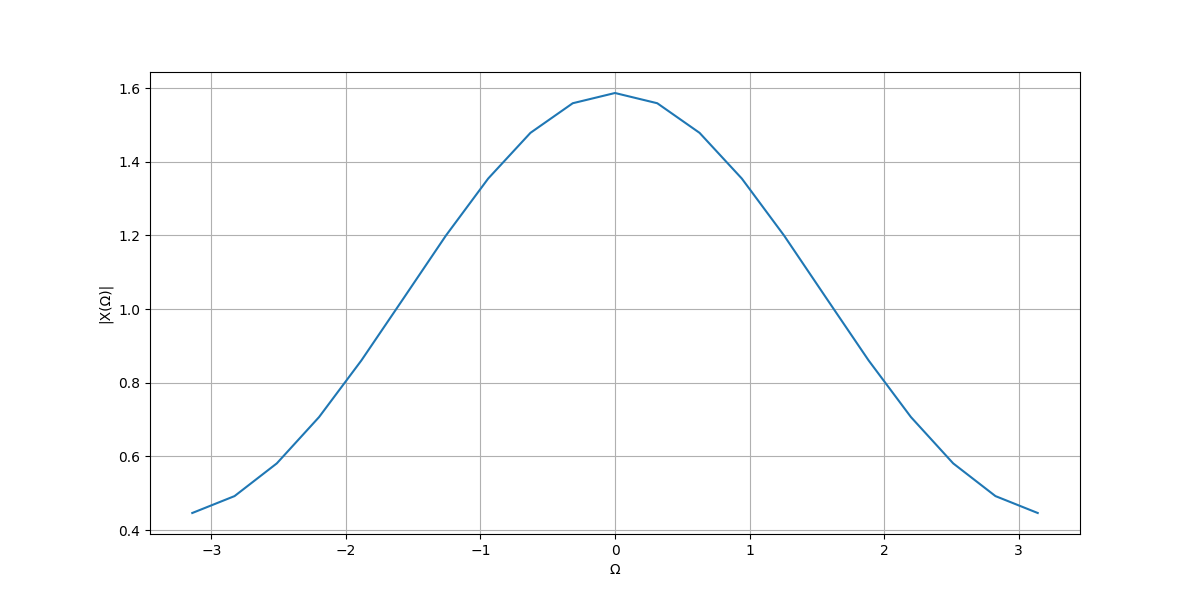
\includegraphics[width=\linewidth]{Imagens/fig15.png}
    \caption{Magnitude para sinal subamostrado a [5n]}
    \label{fig:graph_15}
\end{figure}

Por fim, os efeitos da subamostragem são novamente vistos na representação do sinal subamostrado em fase. Assim, as distorções se intensificaram mais ainda.

\begin{figure}[!htb]
    \centering
    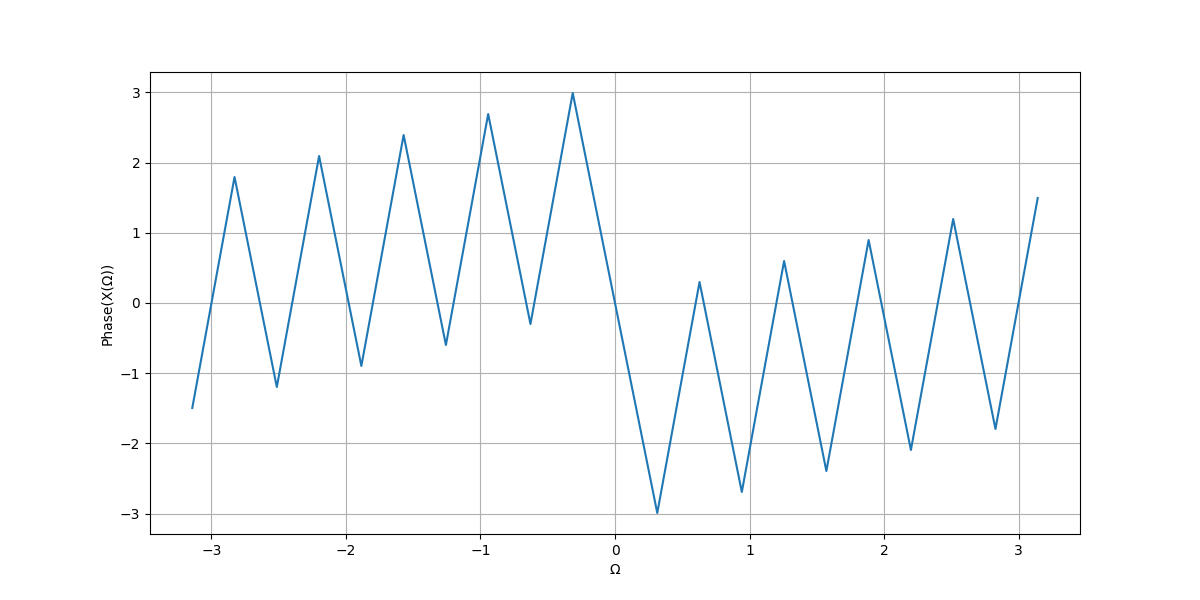
\includegraphics[width=\linewidth]{Imagens/fig16.png}
    \caption{Fase para sinal subamostrado a [5n]}
    \label{fig:graph_16}
\end{figure}

Portanto, as análises dessa questão possibilitaram visualizar os efeitos de uma subamostragem tanto na representação em magnitude quanto em fase. Além disso, esses efeitos podem ser explicados pela intensificação do \textit{aliasing} produzido por uma taxa de amostragem cada vez menor, que realiza a aproximação de cópias de espectros adjacentes. 
